\documentclass{article}
\usepackage{graphicx} % Required for inserting images
\documentclass{article}
\usepackage{amsmath}
\usepackage{amssymb}
\usepackage[utf8]{inputenc}
\usepackage{amsmath}
\usepackage{amssymb}
\usepackage{authblk}
\usepackage{setspace}
\usepackage[margin=1.25in]{geometry}
\usepackage{graphicx}
\graphicspath{ {./figures/} }
\usepackage{subcaption}
\usepackage{amsmath}
\usepackage{lineno}
\usepackage{hyperref}
\usepackage{comment}
\usepackage{lipsum}

\usepackage{xcolor}

\newcommand{\highlight}[1]{%
  \colorbox{red!50}{$\displaystyle#1$}}


\usepackage[style=nejm, 
citestyle=numeric-comp,
sorting=none]{biblatex}
\addbibresource{PartIIIProjectTemplate.bib}


\title{Project Progress Notebook}
\author{PRABHODA C S}
\date{December 2024}

\begin{document}

\maketitle

\section{Variable translation from Salvio to Barker}  \label{Section 1}
Silvio \cite{Salvio_2022} and especially \cite{Pradisi_2022}, give us for the potential

\begin{equation}
    U(\omega) = \frac{1}{4 c'} \left[ \frac{M_{p}^{2}}{4} \text{sinh}(\text{X}(\omega)) - \beta  \right]^2
\end{equation}
where
\begin{equation}
    \text{X}(\omega) = \sqrt{\frac{2}{3}} \frac{\omega}{M_{p}} + \text{tanh}^{-1} \left(\frac{4 \beta}{\sqrt{M_{p}^{4}+16 \beta^2}} \right)
\end{equation}

Differentiating $U(\omega)$ and setting it equal to zero gives us that 

\begin{equation}
    \omega_{min} = \sqrt{\frac{2}{3}} M_p \left[ \text{sinh}^{-1}\left(\frac{4\beta}{M_{p}^{2}}\right) - \text{tanh}^{-1}\left(\frac{4\beta}{\sqrt{M_{p}^{4} + 16\beta^2}}\right) \right]
\end{equation}

Inserting $\text{ArcSinh(x)} = \ln(x + \sqrt{x^2 + 1})$ and $\text{ArcTanh(x)} = \frac{1}{2} \ln\left(\frac{1+x}{1-x}\right)$, gives us $\omega_{min} = 0$ always.
\\
Barker \cite{barker2024poincaregaugetheoryconformal} gives us potential

\begin{equation}
    U(\varphi) = \frac{\mu^2 \phi_{0}^{4}}{2} \left[ \frac{\sigma}{2} + \sqrt{\nu - \frac{\sigma^2}{4}} \text{sinh}\left( \text{X}(\varphi) \right)  \right]
\end{equation}
where
\begin{equation}
    \text{X}(\varphi) =  \frac{\varphi}{\phi_0 \sqrt{\nu - \frac{\sigma^2}{4}}} - \frac{c}{\phi_0 \sqrt{\nu - \frac{\sigma^2}{4}}}
\end{equation}

\subsection{Translating Variables}   \label{Section 1.1}
We know that, $[\beta] = [M_{p}^{2}]$  and $[c'] = 0$ from \cite{Pradisi_2022}. If we want $\varphi = \omega$ (it can't be $\varphi = f(\omega)$ as that would ruin the $(\partial\varphi)^2$ term in Lagrangian), we are forced to make the substitutions that make dimensional sense:

\begin{align}
    \phi_0 &= \sqrt{\frac{3}{2}} M_p \label{eq:A} \\
    \mu &= \frac{1}{6 \sqrt{2 c'}} \label{eq:B} \\
    \sigma &= -\frac{8 \beta}{M_{p}^{2}} \label{eq:C} \\
    \nu &= 1 + \frac{16 \beta^2}{M_{p}^{4}} \label{eq:D} \\
    c  &= -\sqrt{\frac{3}{2}} M_{p} \text{tanh}^{-1} \left(\frac{4 \beta}{\sqrt{M_{p}^{4}+16 \beta^2}} \right) \label{eq:E}
\end{align}

Now, $[\phi_0] = [c] = [M_p]$ and the rest, $[\mu] = [\sigma] = [\nu] = 0$, to be fair, we can include a term $g^{-1}$ in front of the sinh term in $\text{X}(\omega)$, s.t., $[g] = 0$, the resulting eqns are:

\begin{align}
    \phi_0 &= g \sqrt{\frac{3}{2}} M_p \label{eq:A} \\
    \mu &= g^{-1} \frac{1}{6 \sqrt{2 c'}} \label{eq:B} \\
    \sigma &= - g^{-1} \frac{8 \beta}{M_{p}^{2}} \label{eq:C} \\
    \nu &= g^{-2} \left( 1 + \frac{16 \beta^2}{M_{p}^{4}} \right) \label{eq:D} \\
    c  &= -\sqrt{\frac{3}{2}} M_{p} \text{tanh}^{-1} \left(\frac{4 \beta}{\sqrt{M_{p}^{4}+16 \beta^2}} \right) \label{eq:E}
\end{align}

We can see that in \ref{eq:A}, the field $\varphi$ has no dependence on any parameter/is not free, but is fixed by the Planck mass (in Planck units, it is 1.225).

What we can see from equations \ref{eq:A} to \ref{eq:E}, is that $\phi_0 \propto M_p$, with the constant $g$ dictating what fraction of $M_p$,  $\phi_0$ is. $\mu$ is fixed by the strength of coupling of the $\mathcal{R'}^2$ term ($c'$) in the \cite{Pradisi_2022} paper. $c$ is now no longer free and based on the results from \ref{Section 1}, we see that the minima of the potential must now always stay at $\phi_{min} = 0$.

Below is a plot of the aligned graphs with $M_p = 1$ and the values of the parameters upon translation labelled. $g = \sqrt{\frac{1}{3}}$ so that $\phi_0 < M_p$ also.

\begin{figure}[h!]
    \centering
    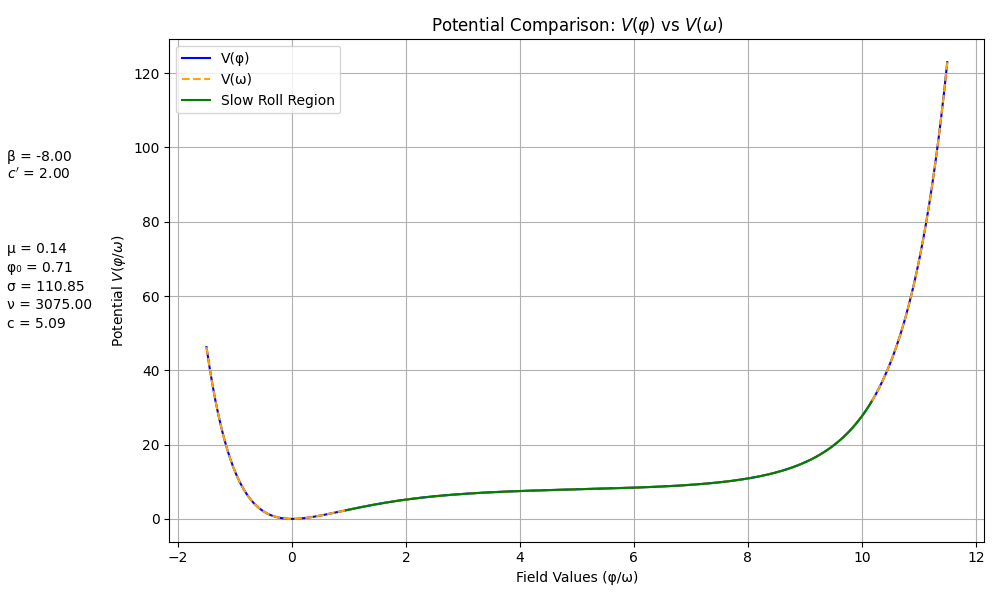
\includegraphics[width=1\textwidth]{Comparing Silvio - Barker.png}
    \caption{Aligned graphs with parameter values on the side}
    \label{Aligned Potential}
\end{figure}

\begin{figure}[h!]
    \centering
    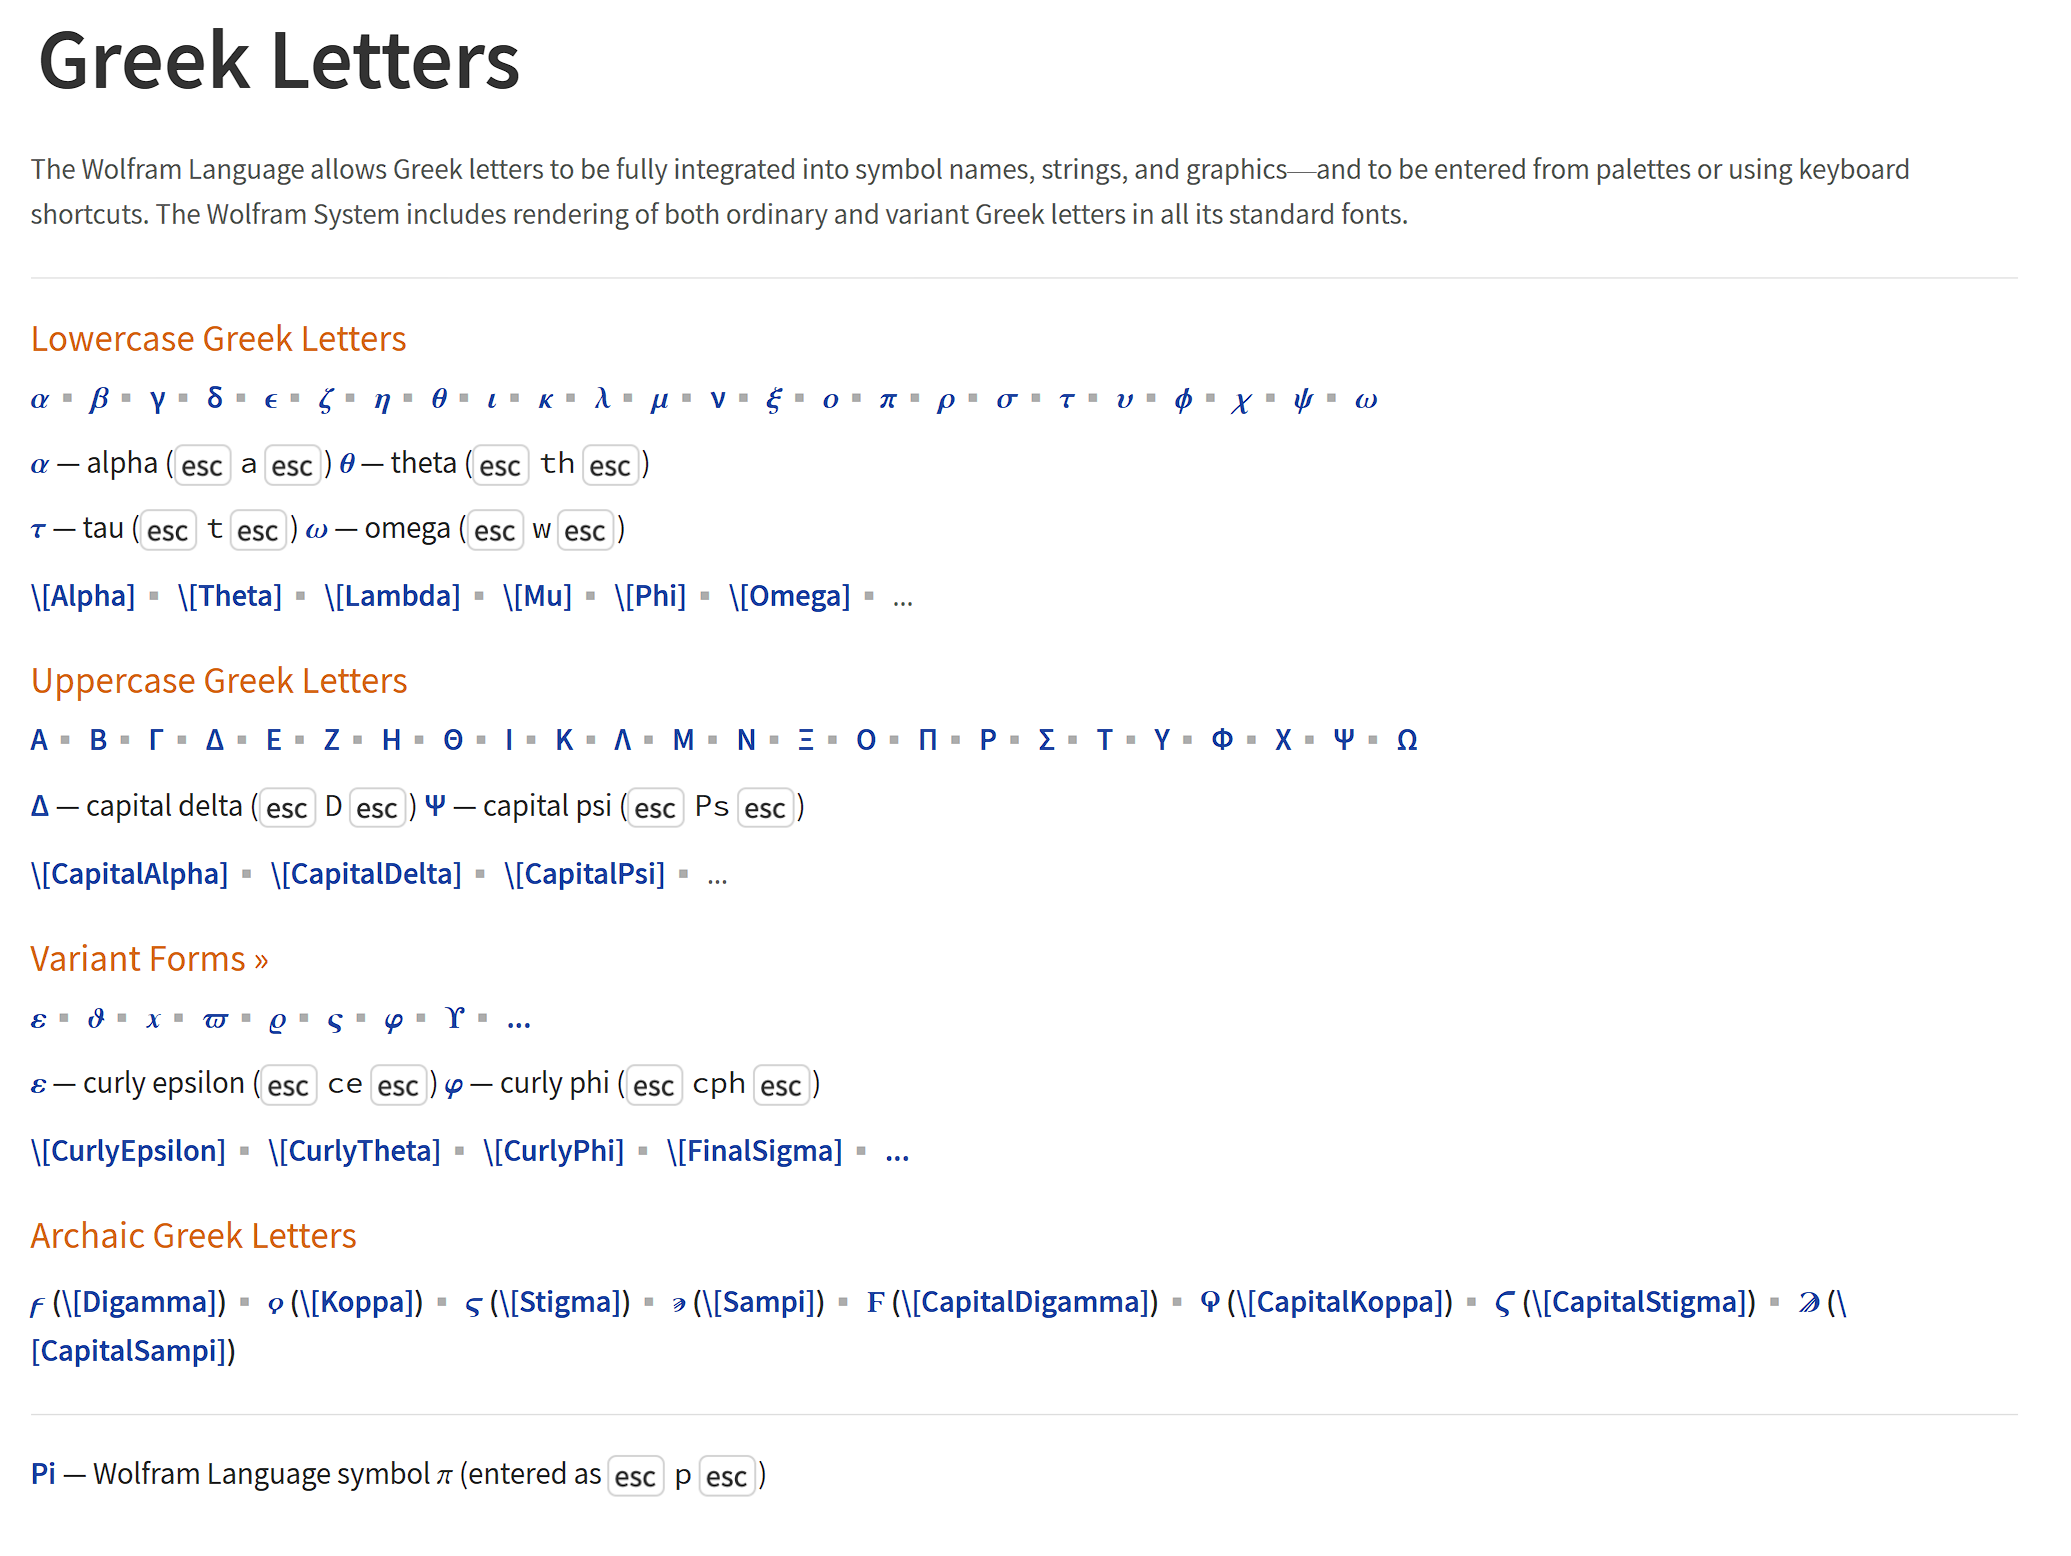
\includegraphics[width=0.8\textwidth]{Insert greek in mathematica.png}
    \caption{Personal Ref}
    \label{Greek in Mathematica}
\end{figure}

For this value of $\beta$, we get $N = 73.582$ as the number of e-folds.

\newpage

\newpage
\section{Coupling to gravity}


To find invariant form of Ricci scalar, look at Christoffel symbol. Can be offset by defining


\begin{equation}
    \mathcal{T}^{\alpha}_{\beta \gamma} = \Gamma^{\alpha}_{\beta \gamma} + (\delta^{\alpha}_{\beta} B_{\gamma} + \delta^{\alpha}_{\gamma} B_{\beta} - g_{\beta \gamma}g^{\alpha \tau}B_{\tau})
\end{equation}

where $B_{\mu} \rightarrow B_{\mu} - \partial_{\mu} \rho$ under a conformal transformation like in \cite{barker2024poincaregaugetheoryconformal}, 

Using this new conformally covariant connection in the definition of the Riemman tennsor and contracting to get conformally covariant Ricci Scalar (CCRS), we get 


\begin{equation}
    \tilde{R} = R - 6 B_{\mu} B^{\mu} - 6 \nabla_\mu B^\mu
\end{equation}

Under a conformal transformation $g_{\mu\nu} \rightarrow e^{2\rho}g_{\mu\nu}$, $\tilde{R} \rightarrow e^{-2\rho} \tilde{R}$
So lagrangian is ? ? 

Literature is out! Since mass scale $\phi$ (Compensator scalar) introduces fundamental scale (as seen in prev section \ref{Section 1.1}, $\phi_0 \sim M_p$), maybe first couple it directly to CCRS, gives us an action in the Jordan Frame, then, transform to Einstein frame, and then minimally couple to inflaton field $\varphi$ in the PHYSICAL Einstein Frame?

\begin{equation}
    \mathcal{L} = (\alpha \phi^2 + \beta \varphi^2 + \gamma \phi \varphi) \tilde{R} + \frac{\epsilon}{2} D_{\mu}\varphi D^{\mu}\varphi + \frac{\sigma}{2} D_{\mu}\varphi D^{\mu}\phi  +  \frac{\nu}{2} D_{\mu}\phi D^{\mu}\phi - \frac{\mu^2}{2} \phi^2 \varphi^2 - \frac{\xi}{16} H_{\mu\nu}H^{\mu\nu}
\end{equation}

\begin{equation}
    \begin{aligned}
        \mathcal{L} = &\; (\alpha \phi^2 + \beta \varphi^2 + \gamma \phi \varphi)R - 6((\alpha \phi^2 + \beta \varphi^2 + \gamma \phi \varphi)(B_{\mu} B^{\mu} - \nabla_\mu B^\mu) \\
        & +\frac{\epsilon}{2} D_{\mu}\varphi D^{\mu}\varphi + \frac{\sigma}{2} D_{\mu}\varphi D^{\mu}\phi + \frac{\nu}{2} D_{\mu}\phi D^{\mu}\phi \\
        & - \frac{\mu^2}{2} \phi^2 \varphi^2 - \frac{\xi}{16} H_{\mu\nu}H^{\mu\nu}
    \end{aligned}
\end{equation}


Taking a leaf out of \cite{barker2024poincaregaugetheoryconformal}, we pick a gauge choice $g_{\mu \nu} \rightarrow \frac{\phi_0}{\phi} g_{\mu \nu}$, $\varphi \rightarrow \frac{\phi}{\phi_0} \varphi$ and $B_{\mu} \rightarrow B_{\mu} - \partial_{\mu} ln(\phi)$. So that, the resulting action (still in jordan frame)

\begin{equation}
    \begin{aligned}
        \mathcal{L} &= (\alpha \phi^2_0 + \beta \varphi^2 + \gamma \phi_0 \varphi) (R - 6B_{\mu} B^{\mu} - 6\nabla_\mu B^\mu) \\
        &+ \frac{\epsilon}{2} (\partial_\mu \varphi - (\varphi + \frac{\sigma}{\epsilon} \phi_0)B_\mu)(\partial^\mu \varphi - \varphi B^\mu)\\
        &- \frac{\mu^2}{2} \phi^2_0 \varphi^2 + \frac{\nu \phi_{0}^{2}}{2} B_\mu B^\mu - \frac{\xi}{16} H_{\mu\nu}H^{\mu\nu}
    \end{aligned}
\end{equation}

Assuming $\xi << 1$ again or other conditions based on result, we solve for Euler-Lagrange Equations for field $B_\mu$ and get:

\begin{equation}
    B_\mu = \frac{1}{2} \partial_\mu \text{ln}(\epsilon \varphi^2 + \sigma \phi_0 \varphi + \nu \phi^2_0 -12 (\alpha \phi^2_0 + \beta \varphi^2 + \gamma \phi_0 \varphi))
\end{equation}

That is.

\begin{equation}
    B_\mu = \frac{1}{2} \partial_\mu \text{ln}((\epsilon - \beta') \varphi^2 + (\sigma - \gamma') \phi_0 \varphi + (\nu - \alpha')\phi^2_0)
\end{equation}

Where, $\alpha' = 12\alpha, \beta' = 12\beta \text{ and } \gamma' = 12 \gamma$

Now inputting that value of $B_\mu$ into the action and plugging through the calculations, we get

\begin{equation}
    \begin{aligned}
        S &= \int \text{d}^4\text{x} \sqrt{-g} [ (\alpha \phi^2_0 + \beta \varphi^2 + \gamma \phi_0 \varphi) R \\
          & - 6 (\alpha \phi^2_0 + \beta \varphi^2 + \gamma \phi_0 \varphi)B_{\mu} B^{\mu} + 6\partial_\mu (\alpha \phi^2_0 + \beta \varphi^2 + \gamma \phi_0 \varphi)B^\mu \\
        &+ \frac{\epsilon}{2} (\partial_\mu \varphi - (\varphi + \frac{\sigma}{\epsilon} \phi_0)B_\mu)(\partial^\mu \varphi - \varphi B^\mu)\\
        &- \frac{\mu^2}{2} \phi^2_0 \varphi^2 + \frac{\nu \phi_{0}^{2}}{2} B_\mu B^\mu - \frac{\xi}{16} H_{\mu\nu}H^{\mu\nu} ] 
    \end{aligned}
\end{equation}

becomes

\begin{equation}
    \begin{aligned}
        S &= \int \text{d}^4\text{x} \sqrt{-g} [ (\alpha \phi^2_0 + \beta \varphi^2 + \gamma \phi_0 \varphi) R \\
        &+ \frac{30 \beta}{2} \left[ 1 - \frac{\phi_0^2}{48\beta V} [(\sigma - 12\gamma)^2 - 4(\epsilon - 12 \beta)(\nu - 12\alpha) ] \right] (\partial_\mu \varphi \partial^\mu \varphi)- \frac{\mu^2}{2} \phi^2_0 \varphi^2 ] 
    \end{aligned}
\end{equation}

where $V = [(\epsilon - 12\beta) \varphi^2 + (\sigma - 12\gamma) \phi_0 \varphi + (\nu - 12\alpha)\phi^2_0]$

Let us reparametrize the metric such that the action takes the form of an Einstein-Hilbert Lagrangian + Matter Lagrangian. For this we choose $g_{\mu\nu} \rightarrow \Omega^2 g_{\mu\nu} $, this makes the  Ricci Scalar go as $\Omega^{-2} [R - 6\frac{\Box\Omega}{\Omega}]$, by setting $\Omega^2 = A^{-1} * M^{-2}$, where $A = (\alpha \phi^2_0 + \beta \varphi^2 + \gamma \phi_0 \varphi)$ and M is the coupling constant (Planck Mass) and something we can use to eliminate one of the 6 variables in our equation and make it simpler. So action becomes

\begin{equation}
    \begin{aligned}
        S &= \int \text{d}^4\text{x} \sqrt{-g} [ \frac{1}{M^2}  R \\
        &+ \Omega^2 \frac{30 \beta}{2} \left[ 1 - \frac{\phi_0^2}{48\beta V} [(\sigma - 12\gamma)^2 - 4(\epsilon - 12 \beta)(\nu - 12\alpha) ] \right] (\partial_\mu \varphi \partial^\mu \varphi) - \frac{3}{2M^2} \frac{(2\beta \varphi + \gamma \phi_0)^2}{(\alpha \phi^2_0 + \beta \varphi^2 + \gamma \phi_0 \varphi)^2} (\partial_\mu \varphi \partial^\mu \varphi)  \\
        &- \Omega^4 \frac{\mu^2}{2} \phi^2_0 \varphi^2 ] 
    \end{aligned}
\end{equation}

which subbing in $\Omega^4$, we get,
\begin{equation}
    \begin{aligned}
        S &= \int \text{d}^4\text{x} \sqrt{-g} [ M^2 R \\
        &+ M^2 \frac{1}{(\alpha \phi^2_0 + \beta \varphi^2 + \gamma \phi_0 \varphi)} \frac{30 \beta}{2} \left[ 1 - \frac{\phi_0^2}{48\beta \highlight{V}} [(\sigma - 12\gamma)^2 - 4(\epsilon - 12 \beta)(\nu - 12\alpha) ] \right] (\partial_\mu \varphi \partial^\mu \varphi)\\ 
        &- \frac{3M^2}{2} \frac{(2\beta \varphi + \gamma \phi_0)^2}{(\alpha \phi^2_0 + \beta \varphi^2 + \gamma \phi_0 \varphi)^2} (\partial_\mu \varphi \partial^\mu \varphi)  \\
        &-  \frac{1}{(\alpha \phi^2_0 + \beta \varphi^2 + \gamma \phi_0 \varphi)^2} \frac{\mu^2}{2} \phi^2_0 \varphi^2 ] 
    \end{aligned}
\end{equation}

where this $V = [(\epsilon - 12\beta) \varphi^2 + (\sigma - 12\gamma) \phi_0 \varphi + (\nu - 12\alpha)\phi^2_0]$ and is the only part which contains the original Barker variables $\{\epsilon, \nu, \sigma \}$, so can't assume Discriminant = 0? Or use this to set other variables?

\newpage

\printbibliography

\end{document}

